% !TEX root = ../thesis-example.tex
%
\chapter{Educational Background}
\label{sec:concepts}

The following quote is attributed to Kurt Lewin --- a pioneer of social psychology: '\emph{Learning is more effective when it is an active rather than a passive process.}'. Being inspired (among others) by the philosophy of Lewin, Kolb presented in 1984 the experiential learning theory~\cite{kolb:1984:experiential}.
This approach features a learning cycle consisting of four learning stages as seen in \autoref{fig:learningCycle}:

\begin{itemize}
    \setlength{\itemsep}{-0.3cm}
    \item Concrete Experience (Experiencing): The learner experiences something here and now which initiates a learning process.
    \item Reflective Observation (Reflecting): During and after the experience observations are made and data is collected.
    \item Abstract Conceptualization (Thinking): The observation and data of the experience is then analyzed and conclusions are drawn.
    \item Active Experimentation (Acting): The learner's behavior is adapted according to conclusions of the analysis to form new experiences. 
\end{itemize}

\begin{figure}[h!bt]
	\centering
	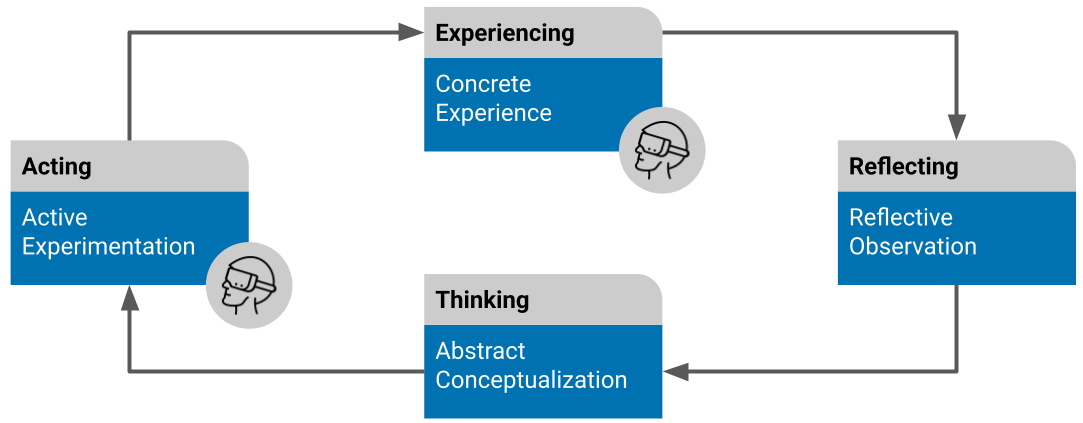
\includegraphics[width=0.9\linewidth]{pictures/ExperientialLearningCycle2.png}
	\captionsetup{labelfont=bf,textfont=it}
	\caption[The Experiential learning cycle as defined by Kolb \cite{kolb:1984:experiential}.]{The Experiential learning cycle as defined by Kolb \cite{kolb:1984:experiential}. Icons mark the stages where \acrshort{xr} could potentially be leveraged the most.\label{fig:learningCycle}}
\end{figure}

Computers can help to shift subjects we are not able to experience first hand (due to cost, risk, geographic distance, or the abstract nature of the topic) into an experiential learning scenario. \Acrfull{xr} can increase this effect additionally due to its often spatial and haptic aspects.
The stages \emph{Concrete Experience} and \emph{Active Experimentation} are particularly suited to carry out in an \acrshort{xr} setting, because of their interactive nature. \acrshort{xr} can increase the interaction and immersion of those stages and therefore raise the impact of these experiences.
As a consequence, several research approaches in the current literature leverage \acrshort{xr} and its subcategories \acrshort{ar}, \acrshort{mr}, and \acrshort{vr} for experiential learning (e.g. \cite{asad2021virtual}, \cite{majgaard2020virtual}, \cite{wang2007experiential}, \cite{pueschel:2013:MRCG}).

Similarly, when learning skills (in contrast to theory), it is crucial to do so in lifelike environments. For example, we learn how to swim in the water and learn how to drive a car on the road. The natural haptics of skill learning makes it a good fit for both, experiential learning and \acrshort{mr}. More detail on skill learning, especially in the context of physical activity, is provided in \autoref{sec:stages}.